% !TEX program = xelatex
\documentclass[
  10pt,
  twoside,
  openany,
  b5paper, % 以上均为 ctexbook 提供的文类选项
  colorscheme = basic, % 请根据需要选择或定制配色方案
]{qyxf-book}
\usepackage{pdfpages}
\usepackage[contents = 钱院学辅, scale = 15, color = black, angle = 50, opacity = .10]{background}
\includepdfset{pagecommand={\thispagestyle{plain}}}

\title{编译器设计专题实验小助手}
\subtitle{Assistant of Compiler Design Lab}  % 可选
\author{本书编写组}
\date{2021 年 1 月 28 日}
%\typo{AlphaGo}  % 排版人员信息,选填

% 定制元信息
\org{\Large\textit{钱学森书院学业辅导中心}\\\textsc{Qian Xuesen College Academic Counseling Center}}
\footorg{\textsc{Qian Yuan Xue Fu}}
\cover{
	\begin{tikzpicture}[remember picture, overlay]
		\begin{pgfonlayer}{background}
			\node at ($(current page.east)+(0in,0in)$){
				
\includegraphics[width=.8\textwidth]{cover.png} };
		\end{pgfonlayer}
	\end{tikzpicture}
}
\license{}  % 清空许可证信息

% 调整封面标题大小
\renewcommand{\titlefont}{\Huge\bfseries}
\renewcommand{\subtitlefont}{\LARGE\itshape}

\begin{document}

\maketitle

\chapter*{前言}
\thispagestyle{empty}

这本小册子是依托钱学森书院学业辅导团发表的针对《编译器设计专题实验》而编写的实验课小助手。编写人员均为2018级计算机系顺利完成该实验的同学。在做实验的过程中,同学们颇感资料匮乏。本实验可以利用的全部资料基本上只有:戴老师的ppt,赵银亮老师2012年的实验指导书(内容残缺不全),斯坦福大学CS143编译原理课程视频(可以上B站寻找),以及网上一些关于Linux系统的博客等资料。ppt在逻辑表述方面有一定的局限性,往往需要听老师讲解才能看懂ppt的意思。18级学生在做该实验时正值2020年新冠肺炎(covid-19)肆虐之时,原有的教学计划被打乱导致上课不便,以至于同学们常常有“学了1+1,就让造飞机”的错觉。

好在新的编译器实验指导书正在编写中。相信随着编译器实验指导书的出版,以上这些问题将很快会迎刃而解。本小助手包含实验环境搭建,常见BUG的解决和基本实验操作,旨在以朋辈的角度帮助学弟学妹们快速入门实验课,节省一些在小问题上耗费的时间,以便把更多的经历投入到实验课核心内容的设计上来。

从18级学生的经验来看,成绩不理想的同学往往都是平时实验任务没有抓紧完成,导致最后一周交报告时手忙脚乱,最终走上抄袭的道路。本实验课程的成绩将会是百分制而不是等级制,抄袭而来的实验报告将会是60~70分,而独立完成的实验报告至少都在85分以上。届时老师会要求大家在报告中提供实验截图,而实验截图中的终端提示符必须包含能够表明自己身份的唯一性标识(参见第一章的修改终端提示符部分)。因此从理论上说抄报告是没有可能的。实际上,18级未改终端提示符的报告均为60~70分,因此平时认真完成每一次实验非常重要。本小助手只提供了基本的实验思路和常见问题的解决,本实验中一切截图中的终端提示符均带有钱院学辅唯一性标识“qyxf”,并且所有内容在公开发表前均交付戴老师审阅。希望能够帮助同学们独立思考并完成实验,在实验思路上能够有所创新和突破。

如前所述,本课程在成绩单上将会是百分制,如何取得好成绩往往是同学们最为关注的问题。2020年ehall更新了成绩查询系统,可以从中看到每门课程成绩的统计数据。我们从该系统看到,本门课程的平均成绩在80分左右,达到85分以上的约有10\%,达到90分以上的约有5\%。无不及格成绩。即便本实验课不会轻易让学生挂科,但是由于本课程是采用百分制的必修课程,虽然只占1学分,不认真做实验也会导致平均学分绩受到极大影响。因此我们再次呼吁同学们杜绝抄袭,独立完成报告。(但是在做实验时可以和其他同学交流合作)

如何拿到90分:

1.	修改终端提示符,杜绝抄袭,完成所有必做实验,按时提交报告:70+

2.	完成所有必做和选做实验,在报告中详述自己完成实验的过程:80+

3.	在实验报告中记录自己遇到的BUG和解决思路:85+

4.	报告内容详实,每次按时完成实验并主动找老师验收:90+

5.	创新实验操作,打通隐藏关卡:???

本小助手编写之时正逢2020新冠肺炎肆虐之际。由于疫情的冲击,实验课只做了前6次实验,而且内容上有大幅度删减。本小助手的编写人员均为学生,难免有很多错误和漏洞。希望我们能够起到抛砖引玉之功效,鼓励学弟学妹们在课余时间完善、修正这本小册子的内容,根据实验课的变化做出相应的调整和创新,以朋辈帮扶的形式薪火相传。

Linux终端操作,第一章,VB增强功能,前言,实验简介,COOL语法简介由计算机钱81杨雨龙编写;第二章和VMware简介由计算机钱81彭光宇编写;第三章由计算机钱81刘奥洋编写;第四章和第六章由计算机钱81孟令涵编写;第五章和Linux双系统由计算机84班班长杨舜磊编写。统稿和组织工作由杨雨龙完成。特别鸣谢戴慧珺老师对于本小助手的指导意见。感谢钱院学辅工作人员电气钱82李浩天的鼎力相助和排版工作,使得本小助手得以顺利付梓。
\thispagestyle{empty}

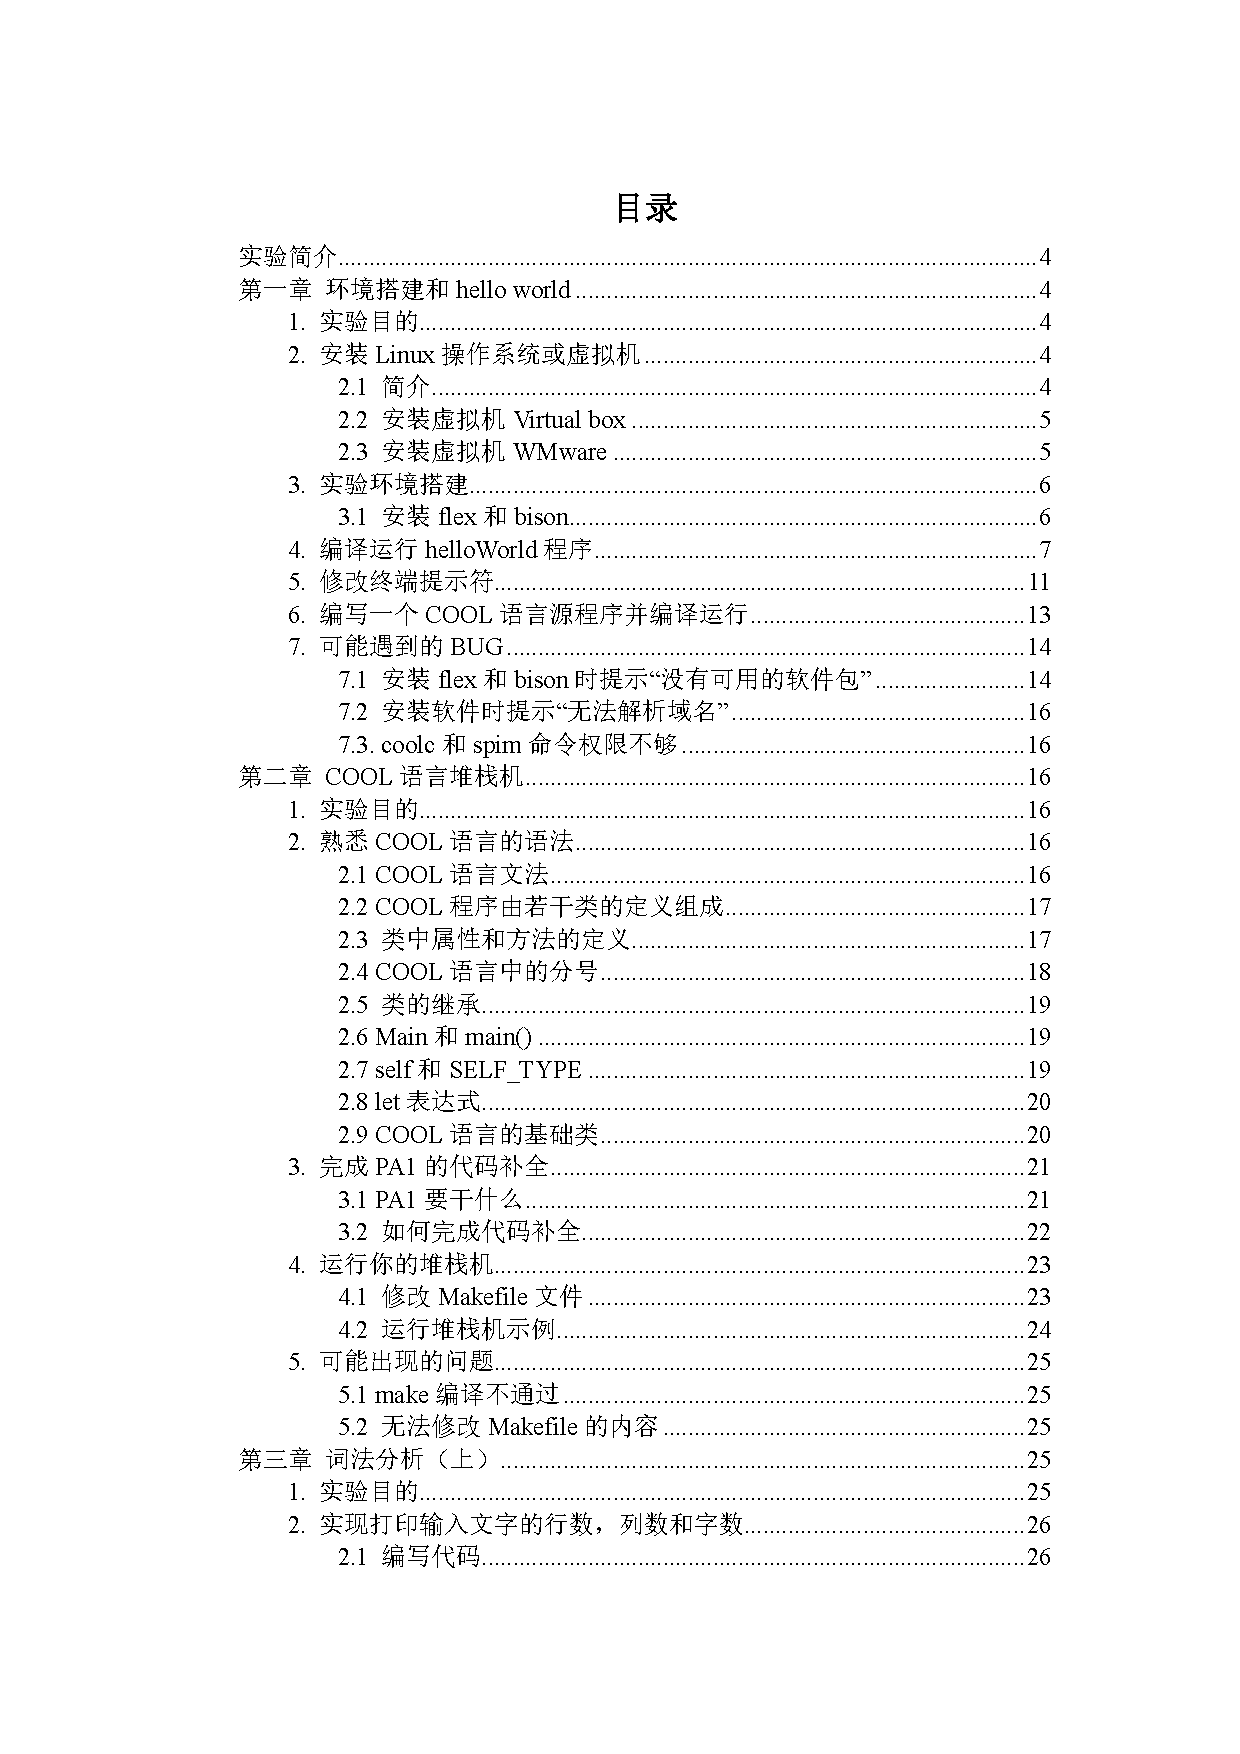
\includepdf[pagecommand = {\thispagestyle{empty}}, pages = - ]{toc.pdf}

\newpage
\setcounter{page}{1}
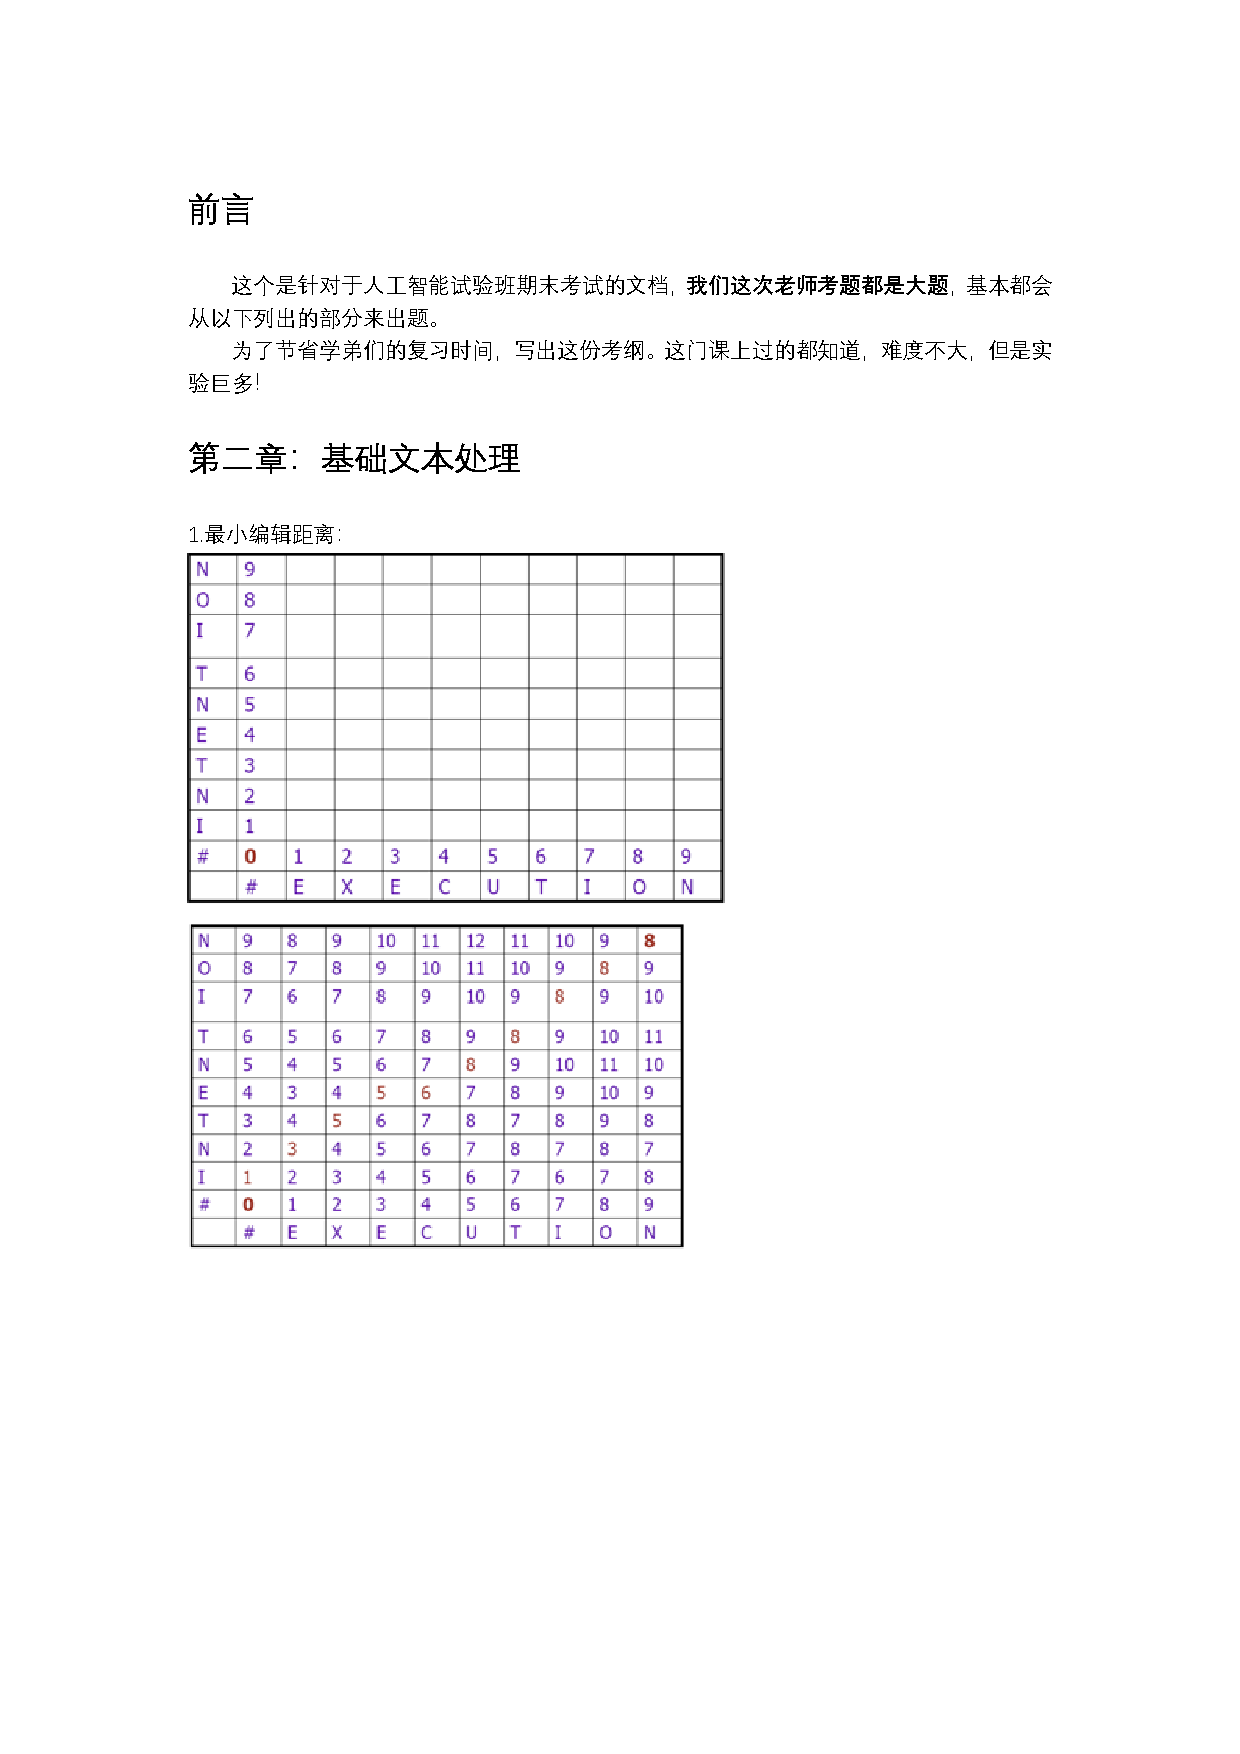
\includepdf[pages = - ]{content.pdf}

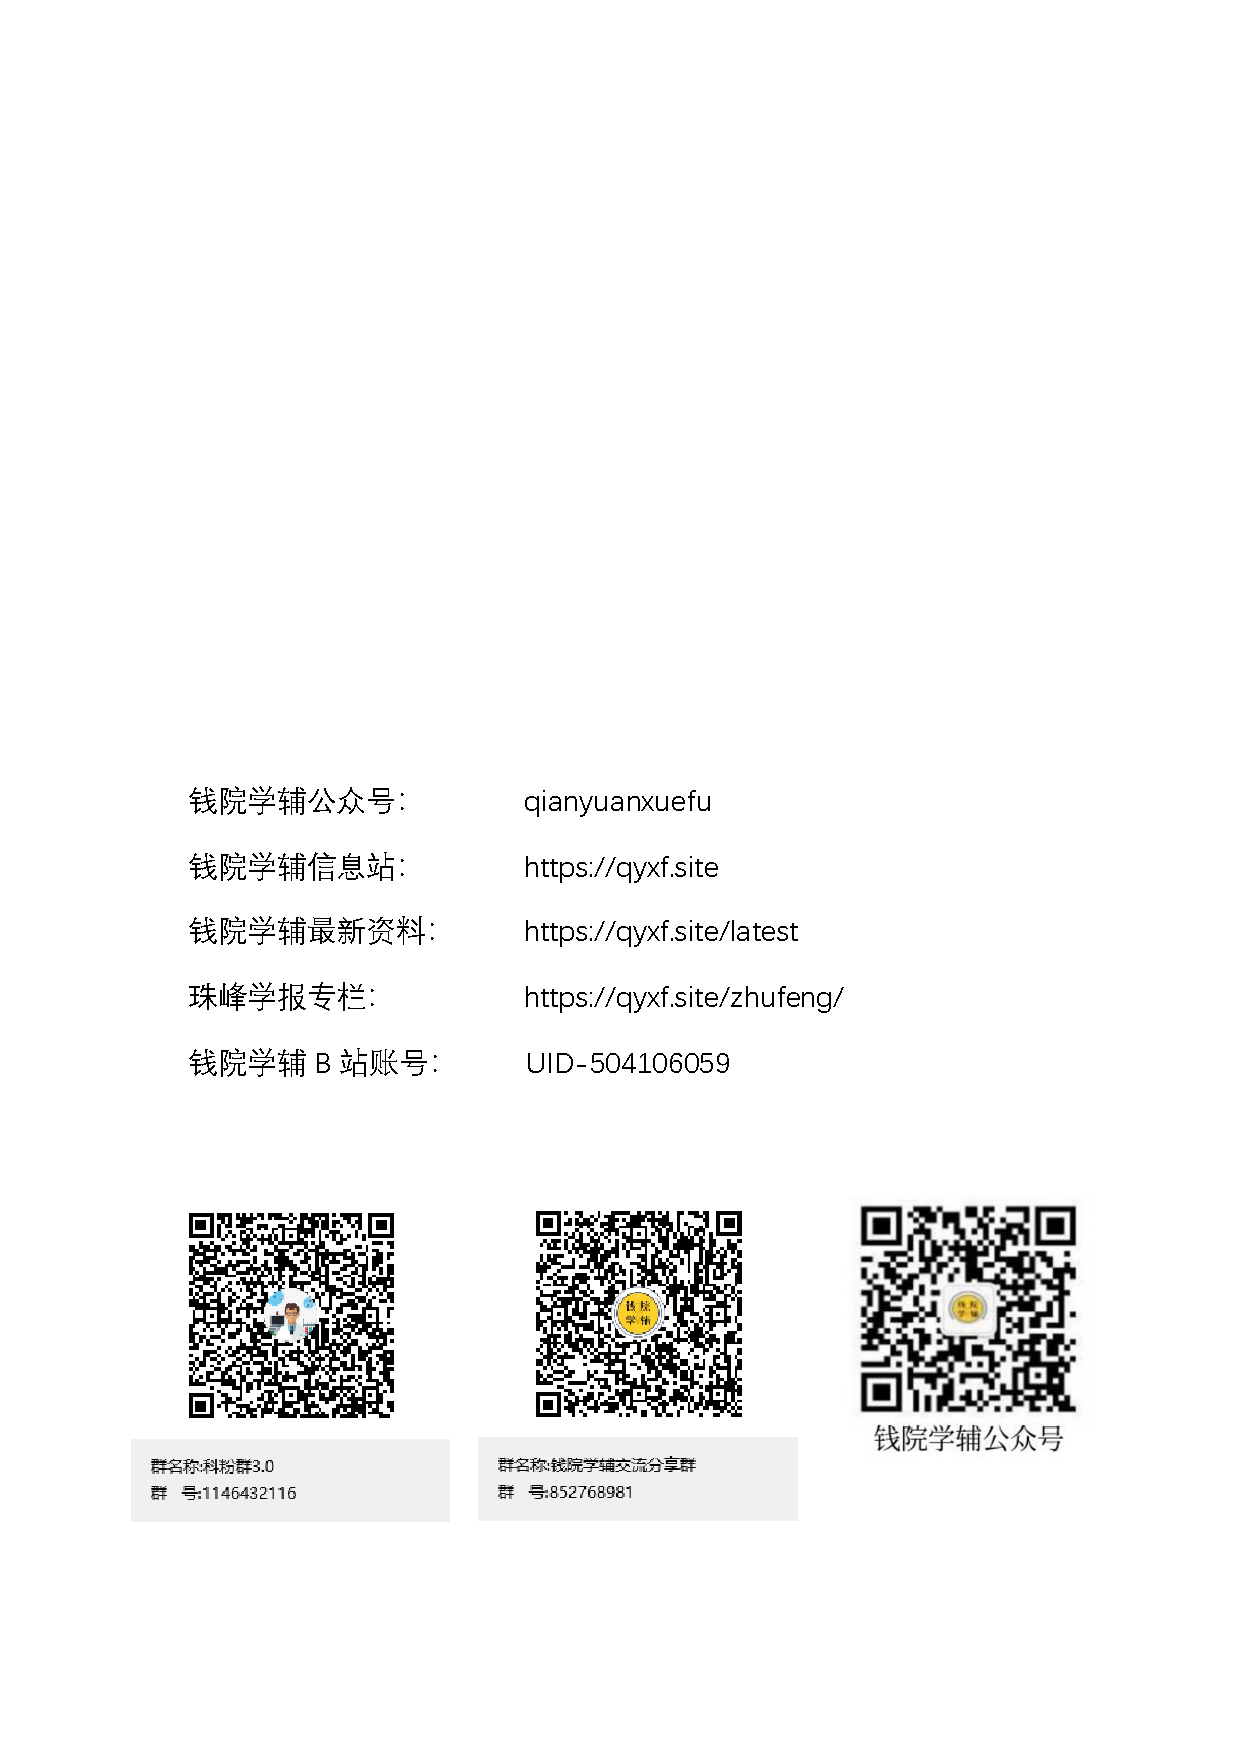
\includepdf[pagecommand = {\thispagestyle{empty}}, pages = - ]{lastpage.pdf}
\end{document}